\section{Versuchsaufbau}

\begin{figure}[h!]
	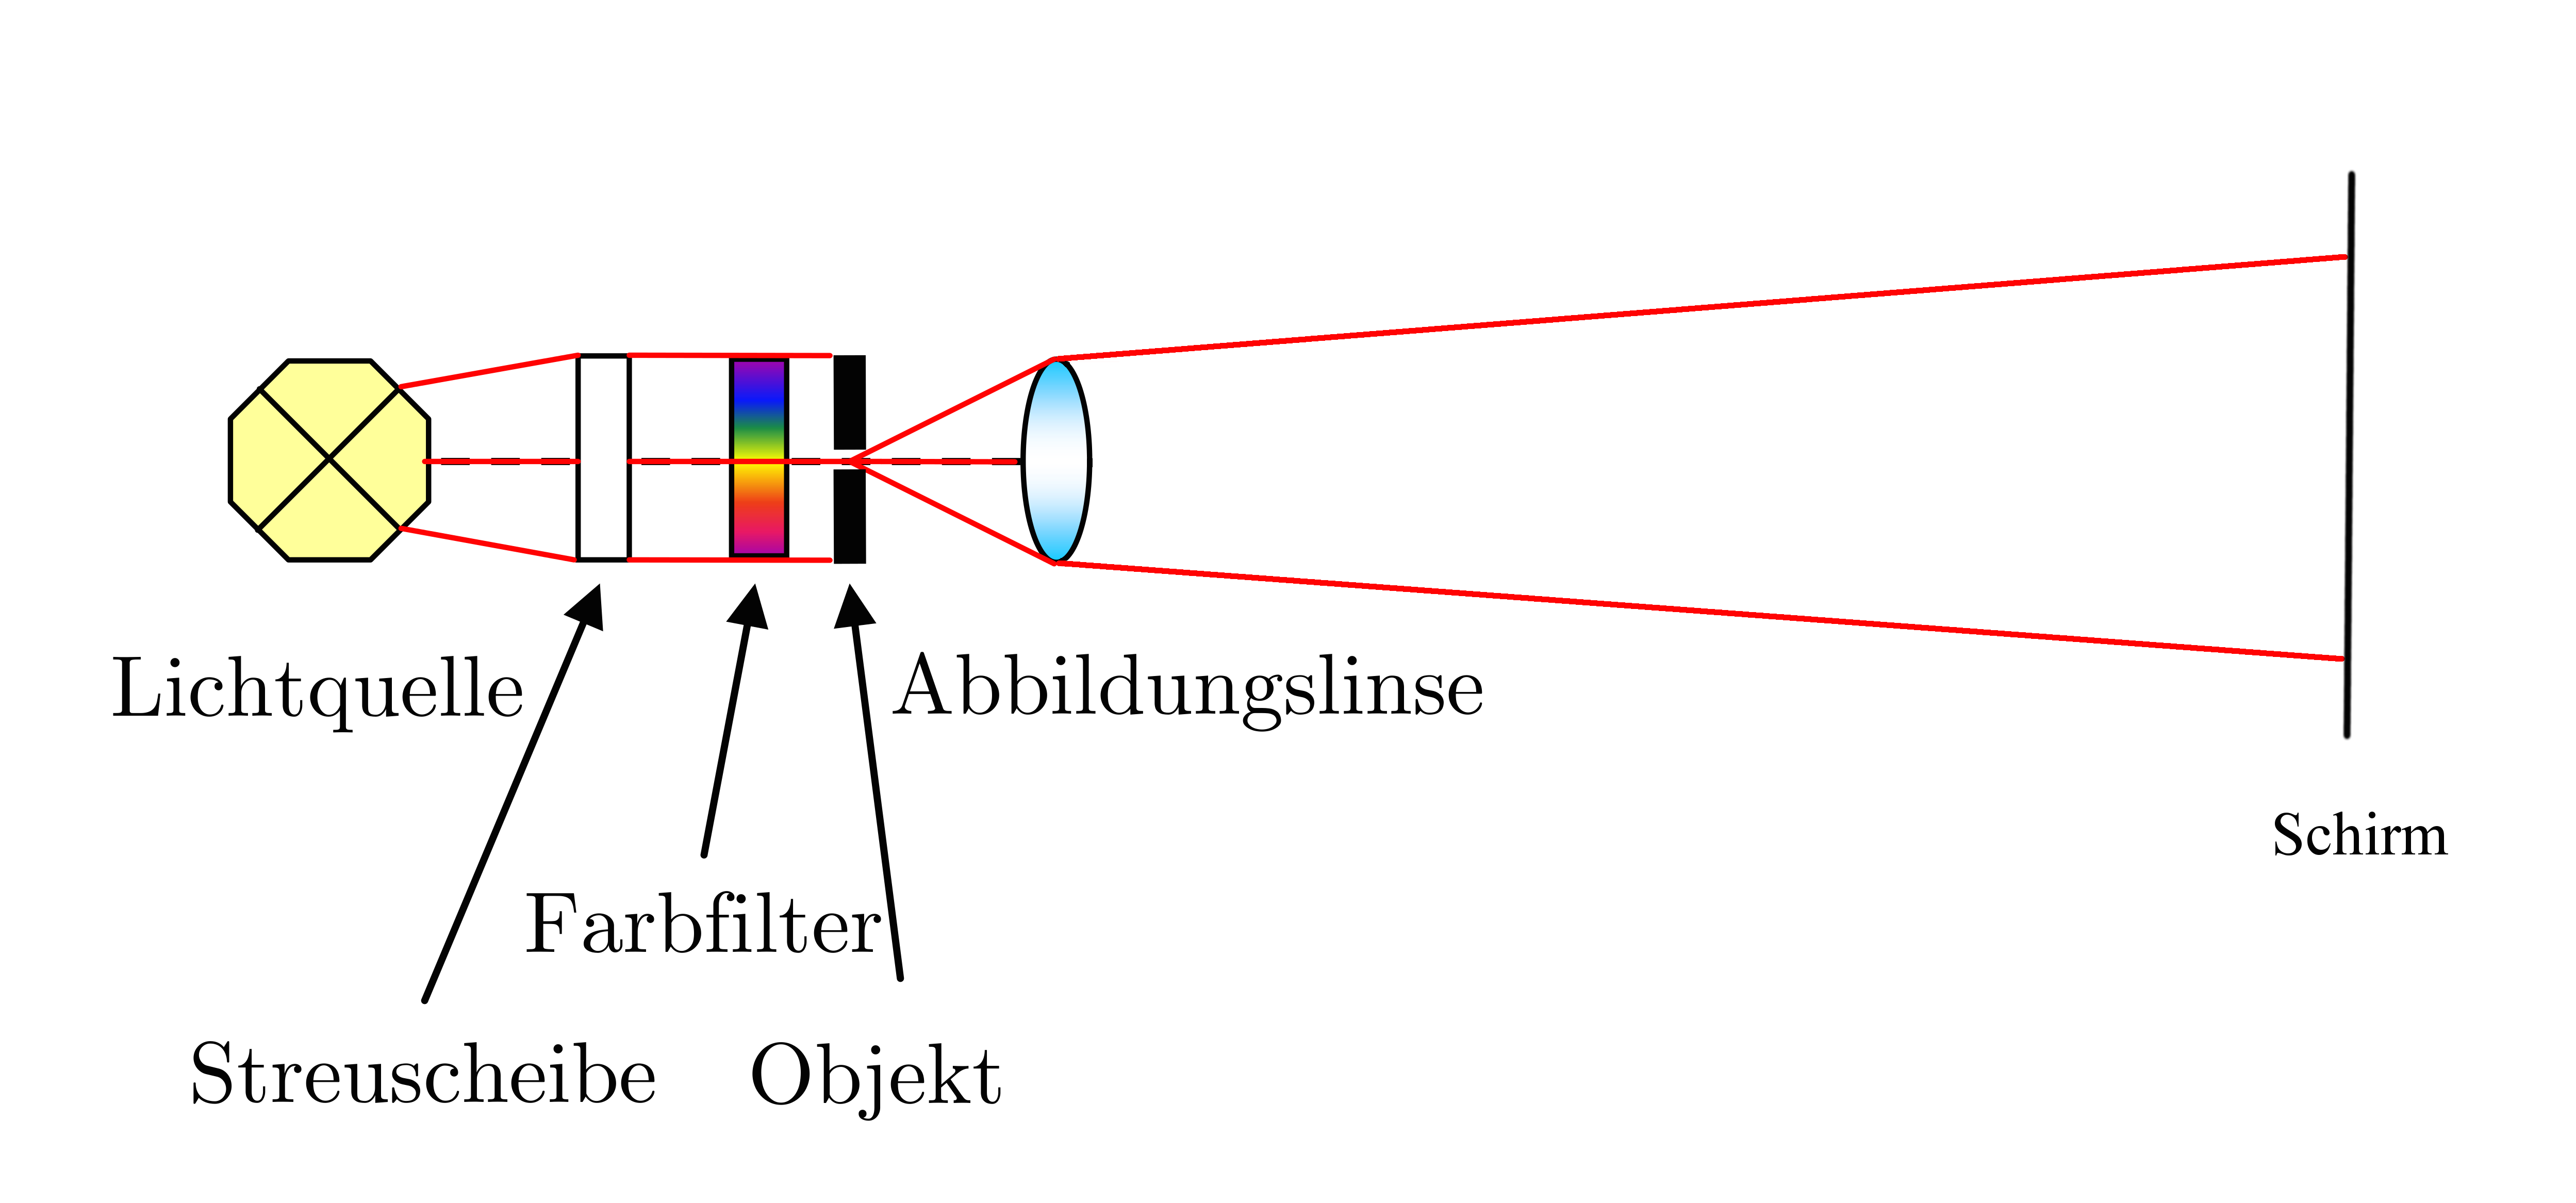
\includegraphics[width=\linewidth]{img/versuchsaufbau.png}
	\caption{Schematischer Versuchsaufbau}
	\label{fig:versuchsaufbau}
\end{figure}

Der Versuchsaufbau wurde mithilfe des Mikro-Bank-Systems Linos realisiert. Der lineare Aufbau bestand aus einer Lichtquelle (Weißlicht), einer Streuscheibe, einem Farbfilter, einem Objekt und einer zu untersuchenden Linse. 

Das Licht der Quelle wurde zuerst in der Streuscheibe gebrochen, um diffuses Licht zu erhalten. Der darauf folgende Farbfilter war einstellbar: Es war sowohl möglich das Licht ungefiltert passieren zu lassen, als auch einen roten, blauen oder grünen Filter anzuwenden. Direkt hinter dem Filter war das Beobachtungsobjekt angebracht. Hierfür eigneten sich beispielsweise ein Siemensstern, eine Skala oder ein grobes Gitter. Hinter dem Objekt wurden Linsen auf das Mikro-Bank-System gesteckt. Diese Linsen zeigten jeweils einen der zu untersuchenden Abbildungsfehler besonders deutlich. Um diesen Fehler sichtbar zu machen, wurde der Fokus über die Position der Linsen eingestellt. 

Die Abbildungen wurden auf einen weißen Papierschirm projiziert, was gegenüber der Verwendung eines CCD-Sensors den Vorteil bot, dass die Abbildungsfehler mit den Augen beobachtet werden konnten. Somit wurde das Auswählen der für den gewünschten Fehler geeignetsten Linse und das Fokussieren vereinfacht.

Nachdem eine für das Protokoll geeignete Abbildung auf dem Schirm realisiert werden konnte, wurde dieser mit einer Spiegelreflexkamera fotografiert. Hierbei war ein manueller Fokus und Weißabgleich zu benutzen.

\begin{figure}[h!]
	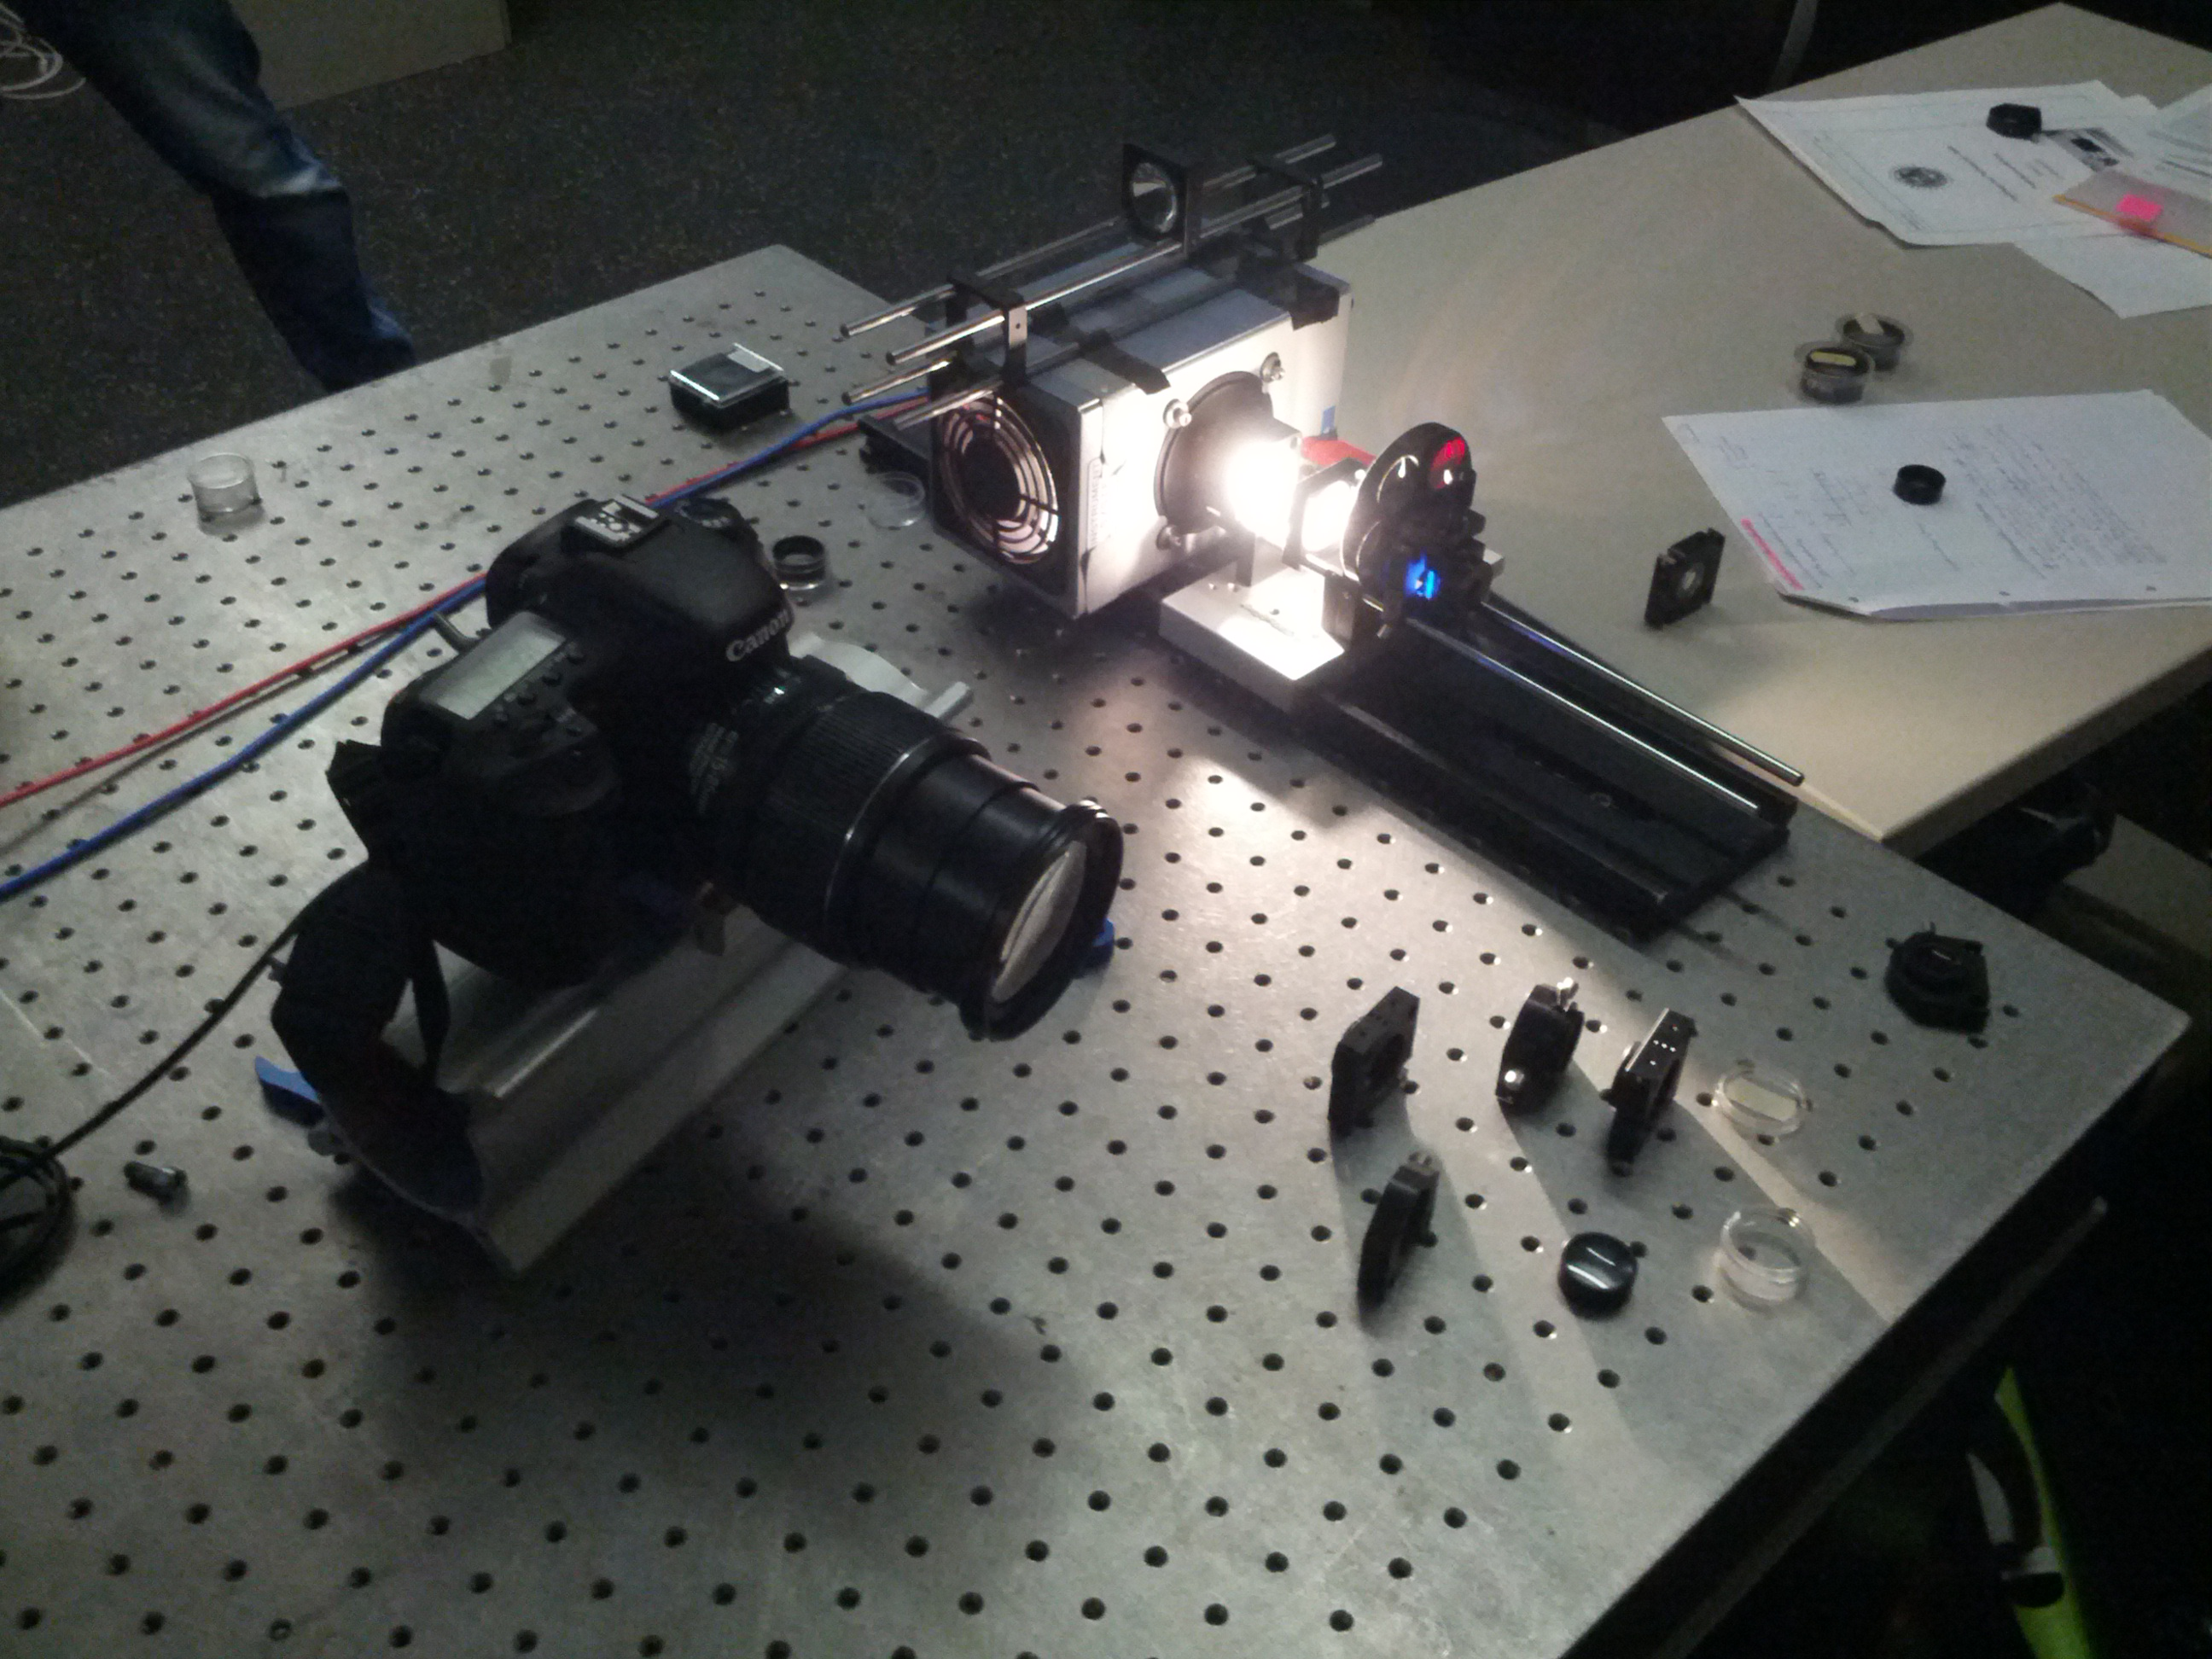
\includegraphics[width=\linewidth]{img/Versuchsaufbau.jpg}
	\caption{Der Versuchsaufbau}
	\label{fig:versuchsaufbaureal}
\end{figure}